\subsection{Mismatched Crowdsourcing}
\label{sec:bgmc}

In~\cite{JHJ15a}, a methodology was proposed that bypasses the need
for native language transcription: mismatched crowdsourcing gives target
language speech to crowd-worker transcribers who have no
knowledge of the target language, then uses explicit mathematical
models of second language phonetic perception to recover an equivalent
phonetic transcription (Fig.~\ref{fig:h2e_eg2}).  Majority voting is
re-cast, in this paradigm, as a form of error-correcting code
(redundancy coding), which effectively increases the capacity of the
noisy channel; interpretation as a noisy channel permits us to explore
more effective and efficient forms of error-correcting codes.

\begin{figure}[b!]\setlength{\textfloatsep}{3mm}
\centerline{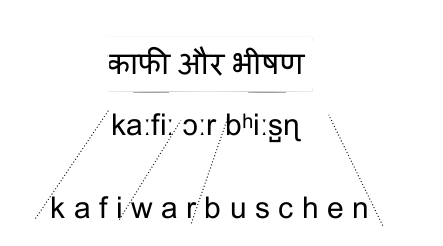
\includegraphics[width=2in]{../figs/h2e_eg1.png}}
\begin{center}
  \tikzstyle{pre2}=[<-,shorten <=3pt,>=stealth',thick, draw=blue]
  \tikzstyle{post2}=[->,shorten >=3pt,>=stealth',thick, draw=blue]
  \begin{tikzpicture}[
      boxed/.style={rectangle,thick, draw=blue, text=black, rounded corners=1mm, fill=orange!35!white, text centered, text width=2.5cm},
      open/.style={text=black, text centered, text width=2.5cm},
    ]
    \node[open] (n0) at (-4,1) {$h$: Utterance-language words};
    \node[boxed] (n1) at (-0.75,1) {Pronunciation FST,\\$\rho(\phi|h)$} 
    edge[pre2](n0);
    \node[boxed] (n2) at (2.5,1) {Misperception FST,\\$\rho(\psi|\phi)$}
    edge[pre2] (n1);
    \node[boxed] (n3) at (5.75,1) {Phoneme-to-grapheme FST, $\rho(\lambda|\psi)$}
    edge[pre2] (n2);
    \node[open] (n4) at (9,1) {$\lambda$: Annotation-language orthography} 
    edge[pre2](n3);
    \node[open] (n5) at (1,-0.35) {$\phi=$Utterance-language phones};
    \node[open] (n6) at (4,-0.35) {$\psi=$Annotation-language phones}; 
  \end{tikzpicture}\\
\end{center}
\setlength{\abovecaptionskip}{0pt}
\caption{Mismatched Crowdsourcing: crowd workers on the web are asked
  to transcribe speech in a language they do not know.  Annotation
  mistakes are modeled by a finite state transducer (FST) model of
  utterance-language pronunciation variability (reduction and
  coarticulation), composed with an FST model of non-native speech
  misperception (mapping utterance-language phones to
  annotation-language phones), composed with an inverted
  grapheme-to-phoneme (G2P) transducer.}
\label{fig:h2e_eg2}
\end{figure}

Assume that cross-language phoneme misperception is a finite-memory
process, and can therefore be modeled by a finite state transducer
(FST).  The complete sequence of representations from utterance
language to annotation language can therefore be modeled as a noisy
channel represented by the composition of up to three consecutive FSTs
(Fig.~\ref{fig:h2e_eg2}): a pronunciation model, a misperception
model, and an inverted grapheme-to-phoneme (G2P) transducer.  The
pronunciation model is an FST representing processes that distort the
canonical phoneme string during speech production, including processes
of reduction and coarticulation.  The misperception model represents
the mapping between the uttered phone string (in symbols matching the
phone set of the spoken language) and the perceived phone string (in
symbols matching the phone set of the annotation language).  Finally,
the transcriber maps heard phones to nonsense words in the annotation
language; the mapping from phones to orthography is an inverted G2P.

Preliminary experiments in mismatched crowdsourcing were carried out
in~\cite{JHJ15a} using Hindi speech excerpts extracted from Special
Broadcasting Service (SBS, Australia) radio podcasts~\cite{SBS}.
Approximately one hour of speech was extracted from the podcasts
(about 10000 word tokens in total) and phonetically transcribed by a
Hindi speaker. The data were then segmented into very short speech
clips (1 to 2 seconds long). The crowd workers were asked to listen to
these short clips and provide English text, in the form of nonsense
syllables, that most closely matched what they heard. The English text
($\lambda$) was aligned with the Hindi phone transcripts ($\phi$)
using a learned transducer, $\rho(\lambda|\phi)$, called a
misperception G2P because it replaces both the misperception and G2P
transducers from Fig.~\ref{fig:h2e_eg2}.  Fig.~\ref{fig:channelfst}
shows a schematic diagram of the misperception G2P, with learned
Levenshtein distances. This FST probabilistically maps each Hindi
phone to either a single English letter or a pair of English
letters. The FST substitution costs, deletion costs and insertion
costs are learned to maximize $\rho(\lambda|\phi)$ using the expectation
maximization algorithm (EM)~\cite{Dempster77}.

\begin{figure}[b!]
\centering
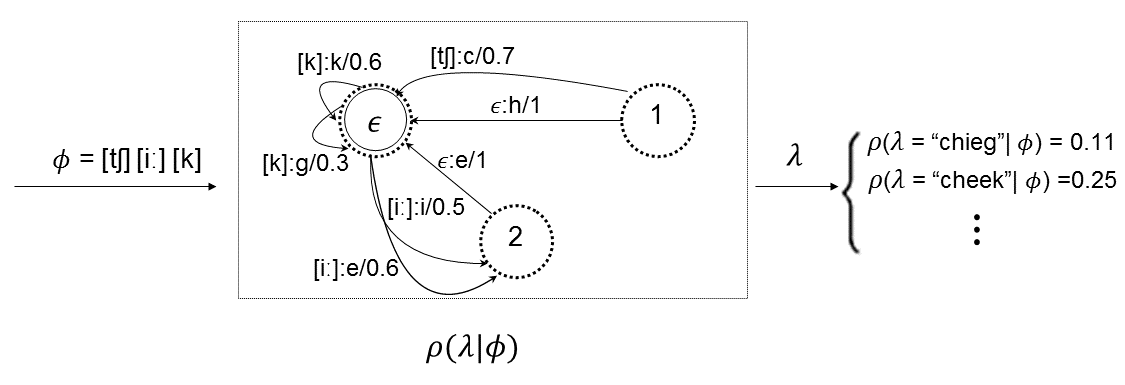
\includegraphics[width=\linewidth]{../figs/mismatchfst.png}
\caption{Mismatch FST model of Hindi transcribed as English.\label{fig:channelfst}}
\end{figure}

